% Created by tikzDevice version 0.12 on 2019-01-03 18:27:37
% !TEX encoding = UTF-8 Unicode
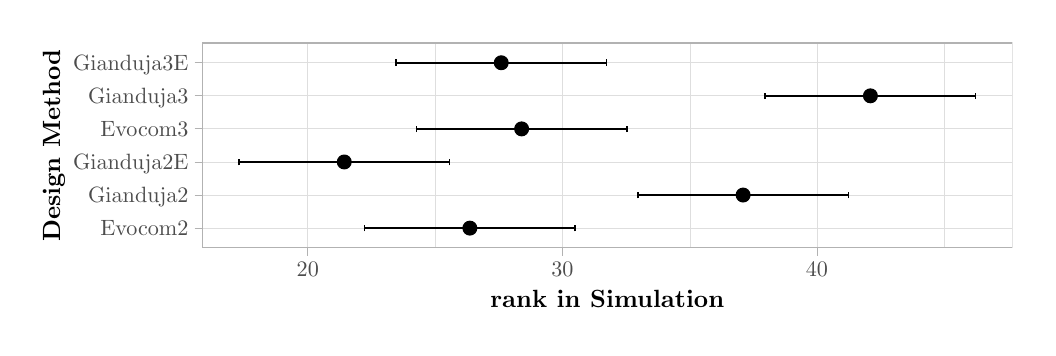
\begin{tikzpicture}[x=1pt,y=1pt]
\definecolor{fillColor}{RGB}{255,255,255}
\path[use as bounding box,fill=fillColor,fill opacity=0.00] (0,0) rectangle (361.35,108.41);
\begin{scope}
\path[clip] (  0.00,  0.00) rectangle (361.35,108.40);
\definecolor{drawColor}{RGB}{255,255,255}
\definecolor{fillColor}{RGB}{255,255,255}

\path[draw=drawColor,line width= 0.6pt,line join=round,line cap=round,fill=fillColor] (  0.00,  0.00) rectangle (361.35,108.40);
\end{scope}
\begin{scope}
\path[clip] ( 63.07, 28.81) rectangle (355.85,102.90);
\definecolor{fillColor}{RGB}{255,255,255}

\path[fill=fillColor] ( 63.07, 28.81) rectangle (355.85,102.90);
\definecolor{drawColor}{gray}{0.87}

\path[draw=drawColor,line width= 0.1pt,line join=round] (147.21, 28.81) --
	(147.21,102.90);

\path[draw=drawColor,line width= 0.1pt,line join=round] (239.20, 28.81) --
	(239.20,102.90);

\path[draw=drawColor,line width= 0.1pt,line join=round] (331.20, 28.81) --
	(331.20,102.90);

\path[draw=drawColor,line width= 0.3pt,line join=round] ( 63.07, 35.98) --
	(355.85, 35.98);

\path[draw=drawColor,line width= 0.3pt,line join=round] ( 63.07, 47.93) --
	(355.85, 47.93);

\path[draw=drawColor,line width= 0.3pt,line join=round] ( 63.07, 59.88) --
	(355.85, 59.88);

\path[draw=drawColor,line width= 0.3pt,line join=round] ( 63.07, 71.83) --
	(355.85, 71.83);

\path[draw=drawColor,line width= 0.3pt,line join=round] ( 63.07, 83.78) --
	(355.85, 83.78);

\path[draw=drawColor,line width= 0.3pt,line join=round] ( 63.07, 95.73) --
	(355.85, 95.73);

\path[draw=drawColor,line width= 0.3pt,line join=round] (101.21, 28.81) --
	(101.21,102.90);

\path[draw=drawColor,line width= 0.3pt,line join=round] (193.21, 28.81) --
	(193.21,102.90);

\path[draw=drawColor,line width= 0.3pt,line join=round] (285.20, 28.81) --
	(285.20,102.90);
\definecolor{drawColor}{RGB}{0,0,0}
\definecolor{fillColor}{RGB}{0,0,0}

\path[draw=drawColor,line width= 0.4pt,line join=round,line cap=round,fill=fillColor] (159.78, 35.98) circle (  2.50);

\path[draw=drawColor,line width= 0.4pt,line join=round,line cap=round,fill=fillColor] (258.52, 47.93) circle (  2.50);

\path[draw=drawColor,line width= 0.4pt,line join=round,line cap=round,fill=fillColor] (114.40, 59.88) circle (  2.50);

\path[draw=drawColor,line width= 0.4pt,line join=round,line cap=round,fill=fillColor] (178.49, 71.83) circle (  2.50);

\path[draw=drawColor,line width= 0.4pt,line join=round,line cap=round,fill=fillColor] (304.52, 83.78) circle (  2.50);

\path[draw=drawColor,line width= 0.4pt,line join=round,line cap=round,fill=fillColor] (171.13, 95.73) circle (  2.50);

\path[draw=drawColor,line width= 0.6pt,line join=round] (197.80, 34.78) --
	(197.80, 37.17);

\path[draw=drawColor,line width= 0.6pt,line join=round] (197.80, 35.98) --
	(121.76, 35.98);

\path[draw=drawColor,line width= 0.6pt,line join=round] (121.76, 34.78) --
	(121.76, 37.17);

\path[draw=drawColor,line width= 0.6pt,line join=round] (296.54, 46.74) --
	(296.54, 49.13);

\path[draw=drawColor,line width= 0.6pt,line join=round] (296.54, 47.93) --
	(220.50, 47.93);

\path[draw=drawColor,line width= 0.6pt,line join=round] (220.50, 46.74) --
	(220.50, 49.13);

\path[draw=drawColor,line width= 0.6pt,line join=round] (152.42, 58.69) --
	(152.42, 61.08);

\path[draw=drawColor,line width= 0.6pt,line join=round] (152.42, 59.88) --
	( 76.38, 59.88);

\path[draw=drawColor,line width= 0.6pt,line join=round] ( 76.38, 58.69) --
	( 76.38, 61.08);

\path[draw=drawColor,line width= 0.6pt,line join=round] (216.51, 70.64) --
	(216.51, 73.03);

\path[draw=drawColor,line width= 0.6pt,line join=round] (216.51, 71.83) --
	(140.47, 71.83);

\path[draw=drawColor,line width= 0.6pt,line join=round] (140.47, 70.64) --
	(140.47, 73.03);

\path[draw=drawColor,line width= 0.6pt,line join=round] (342.54, 82.59) --
	(342.54, 84.98);

\path[draw=drawColor,line width= 0.6pt,line join=round] (342.54, 83.78) --
	(266.50, 83.78);

\path[draw=drawColor,line width= 0.6pt,line join=round] (266.50, 82.59) --
	(266.50, 84.98);

\path[draw=drawColor,line width= 0.6pt,line join=round] (209.15, 94.54) --
	(209.15, 96.93);

\path[draw=drawColor,line width= 0.6pt,line join=round] (209.15, 95.73) --
	(133.11, 95.73);

\path[draw=drawColor,line width= 0.6pt,line join=round] (133.11, 94.54) --
	(133.11, 96.93);
\definecolor{drawColor}{gray}{0.70}

\path[draw=drawColor,line width= 0.6pt,line join=round,line cap=round] ( 63.07, 28.81) rectangle (355.85,102.90);
\end{scope}
\begin{scope}
\path[clip] (  0.00,  0.00) rectangle (361.35,108.41);
\definecolor{drawColor}{gray}{0.30}

\node[text=drawColor,anchor=base east,inner sep=0pt, outer sep=0pt, scale=  0.80] at ( 58.12, 33.22) {Evocom2};

\node[text=drawColor,anchor=base east,inner sep=0pt, outer sep=0pt, scale=  0.80] at ( 58.12, 45.18) {Gianduja2};

\node[text=drawColor,anchor=base east,inner sep=0pt, outer sep=0pt, scale=  0.80] at ( 58.12, 57.13) {Gianduja2E};

\node[text=drawColor,anchor=base east,inner sep=0pt, outer sep=0pt, scale=  0.80] at ( 58.12, 69.08) {Evocom3};

\node[text=drawColor,anchor=base east,inner sep=0pt, outer sep=0pt, scale=  0.80] at ( 58.12, 81.03) {Gianduja3};

\node[text=drawColor,anchor=base east,inner sep=0pt, outer sep=0pt, scale=  0.80] at ( 58.12, 92.98) {Gianduja3E};
\end{scope}
\begin{scope}
\path[clip] (  0.00,  0.00) rectangle (361.35,108.41);
\definecolor{drawColor}{gray}{0.70}

\path[draw=drawColor,line width= 0.3pt,line join=round] ( 60.32, 35.98) --
	( 63.07, 35.98);

\path[draw=drawColor,line width= 0.3pt,line join=round] ( 60.32, 47.93) --
	( 63.07, 47.93);

\path[draw=drawColor,line width= 0.3pt,line join=round] ( 60.32, 59.88) --
	( 63.07, 59.88);

\path[draw=drawColor,line width= 0.3pt,line join=round] ( 60.32, 71.83) --
	( 63.07, 71.83);

\path[draw=drawColor,line width= 0.3pt,line join=round] ( 60.32, 83.78) --
	( 63.07, 83.78);

\path[draw=drawColor,line width= 0.3pt,line join=round] ( 60.32, 95.73) --
	( 63.07, 95.73);
\end{scope}
\begin{scope}
\path[clip] (  0.00,  0.00) rectangle (361.35,108.41);
\definecolor{drawColor}{gray}{0.70}

\path[draw=drawColor,line width= 0.3pt,line join=round] (101.21, 26.06) --
	(101.21, 28.81);

\path[draw=drawColor,line width= 0.3pt,line join=round] (193.21, 26.06) --
	(193.21, 28.81);

\path[draw=drawColor,line width= 0.3pt,line join=round] (285.20, 26.06) --
	(285.20, 28.81);
\end{scope}
\begin{scope}
\path[clip] (  0.00,  0.00) rectangle (361.35,108.41);
\definecolor{drawColor}{gray}{0.30}

\node[text=drawColor,anchor=base,inner sep=0pt, outer sep=0pt, scale=  0.80] at (101.21, 18.35) {20};

\node[text=drawColor,anchor=base,inner sep=0pt, outer sep=0pt, scale=  0.80] at (193.21, 18.35) {30};

\node[text=drawColor,anchor=base,inner sep=0pt, outer sep=0pt, scale=  0.80] at (285.20, 18.35) {40};
\end{scope}
\begin{scope}
\path[clip] (  0.00,  0.00) rectangle (361.35,108.41);
\definecolor{drawColor}{RGB}{0,0,0}

\node[text=drawColor,anchor=base,inner sep=0pt, outer sep=0pt, scale=  0.90] at (209.46,  7.44) {\bfseries rank in Simulation};
\end{scope}
\begin{scope}
\path[clip] (  0.00,  0.00) rectangle (361.35,108.41);
\definecolor{drawColor}{RGB}{0,0,0}

\node[text=drawColor,rotate= 90.00,anchor=base,inner sep=0pt, outer sep=0pt, scale=  0.90] at ( 11.71, 65.86) {\bfseries Design Method};
\end{scope}
\end{tikzpicture}
